\documentclass[type=dr, dr=rernat, accentcolor=tud7b,colorbacktitle, bigchapter, openright, twoside, 12pt ]{tudthesis}
%\documentclass[11pt,twoside,a4paper]{article}
\usepackage[english]{babel} 
\usepackage[utf8]{inputenc}
\usepackage{graphicx}
\usepackage{pstricks}
\usepackage{psfrag}
\usepackage{enumerate}
\usepackage{float}
\usepackage{epsfig}
\usepackage{geometry}
\usepackage{subfigure}
\usepackage{rotating}
\usepackage{minitoc}
% \usepackage{dominitoc}
\usepackage{multirow}
\usepackage{listings}
%\usepackage{appendix}
%\usepackage[breaklinks=true]{hyperref}
%\usepackage{breakcites}

%%%% 1 1/2 facher Zeilenabstand:	
\usepackage{setspace}
\onehalfspacing




\begin{document}
\chapter{Treatment Planning for Patients with multiple lung metastases}
\label{chapter:vmm}
\minitoc

\section{Introduction}

Lung cancer is the leading cause of cancer-related death, with approximately 160 000 deaths in the U.S. in 2014 \cite{Siegel2014}. More than half of all patients with lung cancer are diagnosed with stage IV non-small cell lung cancer (NSCLC) \cite{Ramalingam2008, Iyengar2014}.
Prognosis for stage IV NSCLC is poor, with only 12 months median survival after first line chemotherapy \cite{Socinski2013}. 

Stereotactic body radiation treatment (SBRT) shows good results for treating NSCLC \cite{Baumann2009, Fakiris2009, Grutters2010, Ricardi2010, Timmerman2010, Greco2011}. Furthermore, several studies have shown that SBRT can be used in the setting of limited metastatic disease \cite{Rusthoven2009. Villaruz2012, Salama2012, Iyengar2014}. Passive scattering particle therapy has also proved as an effective treatment for NSCLC \cite{Grutters2010, Tsujii2012} and it was shown in Chapter~\cite{PatStudy} that scanned carbon ions (CiT) could also be used as a treatment modality for NSCLC. One of the conclusions of our study in Chapter~\ref{PatStudy} was that patients with multiple metastases would especially benefit from CiT compared to SBRT. However, there were just three patients with multiple metastases in study and single-field uniform optimization (SFUD) was used in treatment planning. Since patients with multiple metastases can present complex geometry, SFUD is limited in treatment planning sense.

Different algorithms were proposed to improve optimization of intensity modulated particle therapy (IMPT), such as objective planning, robust and 4D optimization \textbf{Se ksn?}. While none of the algorithms is exclusive for single target, to our knowledge none was actually
tested for patients with multiple ones. Furthermore, treating tumors in lung with IMPT is still challenging due to the interplay and radiological path length changes, as explained in Section~\textbf{REF}.

Nevertheless, the potential of CiT for treating multiple lung metastases was displayed (see Chapter~\ref{PatStudy}) and a deeper investigation into this topic was made. A state of the art 4D optimization and dose calculation techniques were used to fully asses the potential of CiT as a potential treatment modality for multiple lung metastases.


%A simple geometrical union of target contour in different CT states, geo-ITV, leads to poor 4D dose distribution, when treating moving tumors with particle therapy \cite{Rietzel2010}.

\section{Materials and Methods}

For creation of treatment plans 4D extension of GSI's treatment planning system TRiP98 \cite{Kraemer2000a, Richter2013} was used and modified. A description of modifications and tools used will be given here, 
alongside with patient data and analysis description.

\subsection{Multiple targets}

TRiP98 optimization works on minimizing residual of a nonlinear equation system \cite{Kraemer2000a}. The minimizing function $E(N)$ for particle number $\vec{N}$ goes as:
\begin{equation}
\label{eq-costFunc}
 E(\vec{N}) = \sum_{i\in target} \left( D_{pre}^{i} - D_{act}^{i}(\vec{N})\right) = \sum_{i\in target} \left( D_{pre}^{i} -\sum_{j=1}^n c_{ij}N\right)
\end{equation}

For a CT voxel $i$, $ D_{pre}$ and $D_{act}$ are the prescribed and the actual dose, respectively. The coefficient $c_{ij}$ stands for correlation between dose deposition and field position $j$ at a voxel $i$, with $n$ the number of fields. There is not restriction for the number of targets or fields in the minimizing function, so it can be expanded to:

\begin{equation}
\label{eq-multiCost}
 E(\vec{N}) = \sum_{targets} \sum_{i\in target} \left( D_{pre}^{i} -\sum_{j=1}^n c_{ij}N\right)
\end{equation}

However, the setup of raster points in TRiP98 allowed only one target. This setup was expanded in a way that field was designated to a specific target, as displayed in Fig~\ref{Fig:multiTargets}. 
Raster points for each field are created only around designated target. Contribution from all fields are then calculated in optimization. When a field from one target contributes 
dose to the other target this is taken into account in optimization function, specifically in coefficient $c_{ij}$ in Eq.~\ref{eq-costFunc}. Because the optimization function was not changed, 
all TRiP98 4D functionalities could be used, as explained in next sections.


\begin{figure}[H]
	\begin{center}
		\includegraphics[width=0.8\textwidth]{./Images/multiTargets.png}
		\caption{Multiple targets irradiation. Fields 1 and 2 are designated to target a and fields 3 and 4 to target b. Optimization takes into account all target voxels and contributions from all fields.}
		\label{Fig:multiTargets}
	\end{center}
\end{figure}



\subsection{Optimization techniques}

Investigation of two different optimization techniques to handle range changes in moving tumors was made. For each patient, two sets of plans were created: field-independent ITV (indITV) and 4D optimization (4Dopt). 

\begin{itemize}
\item \textbf{Single-field uniform optimization:}  was created for each field and each target specifically \cite{Rietzel2012}. Afterwards each field was individually optimized on a reference phase (end-inhale) to deliver full dose to target. In the end the particle number in each field was divided by number of fields.

\item \textbf{Field-independet ITV:} A water-equivalent path length ITV (WEPL-ITV) are different for each field, creating unnecessary margins when combining WEPL-ITV from different fields (see Fig.~\textbf{!}a). Graeff et. al proposed a solution to include range margin into the field description itself, instead of creating a bigger PTV \cite{Graeff2012}. Thus, no unnecessary margins are created. Treatment plans were made for all targets with intensity modulated particle therapy (IMPT) on a indITV in reference phase.

\item \textbf{4D Optimization:} IMPT with indITV produces inhomogeneous fields that yield homogeneous dose but only in reference phase. The WEPL can change in different motion phases, leading to inhomogeneous dose.
4Dopt uses WEPL-ITV for raster setup, however the actual optimization is performed on each target voxel in each motion state $k$. The optimization function changes then to \cite{Graeff2012}:

\begin{equation}
\label{eq-multiCost}
E(\vec{N}) = \sum_{k=1}^{m}\sum_{targets(k)} \sum_{i\in target(k)} \left( D_{pre}^{i} -\sum_{j=1}^n c_{ijk}N\right)
\end{equation}

All targets were treated with IMPT and 4D optimization. A subset of motion states 0, 50 and 70\% was used for targets 7a -7d and 8b (see Table~\ref{tab:patdata2}) due to large optimization problem - beside multiple targets, OAR was also included
in motion states \cite{Graeff2012}.



\end{itemize}

Finally, fields, resulting from the two optimization techniques mentioned, were used to calculate 4D doses. The same number of fields and the same field angles were used in both techniques.

\subsection{Patient data}

Treatment plans were created for 8 patients with 2 - 5 lung metastases summing to 24 metastases in total. \textbf{Average?}. Details are given in Table~\ref{tab:patdata2}.
Patients 6 - 8 had at least one OAR closer than 10 mm to one or more CTVs. 

Patients were treated with SBRT at Chamaplimaud Center for the Unknown, Lisbon (Portugal), with different fraction schemes. Number of fractions and doses delivered are given in Table~\ref{tab:patdata2}. 

\begin{table}[H]
	\centering
	%   \footnotesize
	\caption{Target characteristics, with CTV volumes, peak-to-peak motions, fractination schemes and number of fields used for treatment planning. Last column 
	shows if there was an OAR in target vicinity. SA stands for smaller airways and esoph. for esophagus.}
	\begin{tabular}{c|c|c|c|c|c|c}
		\hline\hline
		\multirow{2}{*}{Patient} & \multirow{2}{*}{Target} & \multirow{2}{*}{Volume (cm$^3$)} & Peak-to-peak & Fractination & Number & OAR in \\
		 & & & motion [mm] & scheme & of fields & proximity \\
		\hline
		\multirow{2}{*}{1} & a & 10.2 & 3.4  & \multirow{2}{*}{1 x 24 Gy} & \multirow{2}{*}{2} & \multirow{2}{*}{SA} \\
		 & b & 14.4 & 2.8 &  &  &  \\
		 
		 \hline
		 \multirow{5}{*}{2} & a & 136 & 12  & 3 x 9 Gy & \multirow{3}{*}{2} & Heart\\
		  & b & 12.4 & 2.5  & 1 x 20 Gy &  &\\
		  & c & 123 & 14  & 3 x 9 Gy &  &Heart \\
		 & d & 80.7 & 17  & 1 x 20 Gy & 3  &\\
		 & e & 86.7 & 6.6  & 1 x 20 Gy & 2 & \\
		 \hline
		 \multirow{2}{*}{3} & a & 2.3 & 12  & 1 x 24 Gy & \multirow{2}{*}{2} \\
		 & b & 0.4 & 11.8  & 5 x 7 Gy &  \\
		 \hline
		 \multirow{5}{*}{4} & a & 3.8 & 5.8  & \multirow{5}{*}{1 x 24 Gy} & \multirow{5}{*}{2} \\
		  & b & 4.3 & 0.8  &  & \\
		  & c & 2.7 & 3.4  &  & \\
		  & d & 3.1 & 2.1  &  & \\
		  & e & 0.5 & 0.5  &  & \\
		  \hline
		  \multirow{2}{*}{5} & a & 139 & 0.6 & \multirow{2}{*}{1 x 24 Gy} & 3 \\
		 & b & 9.2 & 2.0  &  & 2 \\
		 \hline
		 \multirow{2}{*}{6} & a & 4 & 9  & 3 x 9 Gy  & 5 & SA, esoph. \\
		 & b & 0.8 & 7.8  & 1 x 24 Gy & 2 \\
		 \hline
		 \multirow{4}{*}{7} & a & 3.4   & 4.4    & \multirow{4}{*}{1 x 24 Gy} & 3  \\
				    & b & 2.4 & 4.4  & & \multirow{3}{*}{2} \\
				    & c & 2.0 & 6.3  & & & \multirow{2}{*}{Heart}\\
				    & d & 2.4 & 6.4  & & \\
		\hline	    
		\multirow{2}{*}{8} & a & 20.6 & 7.4 & \multirow{2}{*}{1 x 24 Gy} & \multirow{2}{*}{4} & \multirow{2}{*}{SA}  \\
		 & b & 27.1 & 6.0  &  &   \\
		 
		
		\hline\hline
% 		\hline\hline
% 		\multirow{2}{*}{Patient} & \multirow{2}{*}{Target} & \multirow{2}{*}{Volume (cm$^3$)} & Peak-to-peak & Fractination & Couch/Gantry \\
% 		 & & & motion [mm] & scheme & angles [deg] \\
% 		\hline
% 		\multirow{2}{*}{1} & a & 10.2 & 3.4  & \multirow{2}{*}{1 x 24 Gy} & 0/40, 90/0 \\
% 		 & b & 14.4 & 2.8 &  & 0/40, -90/0 \\
% 		 
% 		 \hline
% 		 \multirow{5}{*}{2} & a & 136 & 12  & 3 x 9 Gy & -90/124, -90/-56 \\
% 		  & b & 12.4 & 2.5  & 1 x 21 Gy & 90/0, 90/-90 \\
% 		  & c & 123 & 14  & 1 x 9 Gy & -90/124, -90/-56 \\
% 		 & d & 80.7 & 17  & 1 x 21 Gy & 90/90, 90/0, 90/-90 \\
% 		 & e & 86.7 & 6.6  & 1 x 21 Gy & 90/90, 90/-90 \\
% 		 \hline
% 		 \multirow{2}{*}{3} & a & 2.3 & 12  & 1 x 24 Gy & 90/90, 90/-90 \\
% 		 & b & 0.4 & 11.8  & 5 x 7 Gy & -90/90, -90/-90 \\
% 		 \hline
% 		 \multirow{5}{*}{4} & a & 3.8 & 5.8  & \multirow{5}{*}{1 x 24 Gy} & -90/90, -90/-90 \\
% 		  & b & 4.3 & 0.8  &  & 90/35, 90/-145 \\
% 		  & c & 2.7 & 3.4  &  & -90/90, -90/-90 \\
% 		  & d & 3.1 & 2.1  &  & 90/90, 90/-90 \\
% 		  & e & 0.5 & 0.5  &  & 90/90, 90/-90 \\
% 		  \hline
% 		  \multirow{2}{*}{5} & a & 139 & 0.6 & \multirow{2}{*}{1 x 24 Gy} & -90/125, -90/90, -90/0 \\
% 		 & b & 9.2 & 2.0  &  & -90/90, -90/0 -90/-90 \\
% 		 \hline
% 		 \multirow{2}{*}{6} & a & 4 & 9  & 3 x 9 Gy & 90/90, 90/45, 90/0, 90/-45, 90/-90  \\
% 		 & b & 0.8 & 7.8  & 1 x 24 Gy &  -90/105, -90/-75 \\
% 		 \hline
% 		 \multirow{4}{*}{7} & a & 3.4   & 4.4    & \multirow{4}{*}{1 x 24 Gy} & -90/90, -90/0, -90/-90  \\
% 				    & b & 2.4 & 4.4  & &  -90/-60, -90/-90 \\
% 				    & c & 2.0 & 6.3  & &  -90/-90, -90/-129 \\
% 				    & d & 2.4 & 6.4  & &  -90/-90, -90/-129 \\
% 		\hline	    
% 		\multirow{2}{*}{8} & a & 20.6 & 7.4 & \multirow{2}{*}{1 x 24 Gy} & 40/40, 90/90, 90/0, 90/-45 \\
% 		 & b & 27.1 & 6.0  &  & -40/40, -90/90, -90/0, -90/-45 \\
% 		 
% 		
% 		\hline\hline
	\end{tabular}
	\label{tab:patdata2}
\end{table}


\subsection{Treatment planning}

An isotropic margin of 3 mm was added to each CTV to account for uncertanties in treatment delivery. An WEPL-ITV was constructed on the CTV with margins for each individual field, which was than used for optimization (SFUD
and inITV) or for raster setup (4Dopt). SFUD and indITV plans were made on an end-inhale phase of a 4D-CT. Due to large memory demands, targets in each lung were optimized seperately. 
  
The objective for target was 99\% of each target volume should receive at least 100\% of the planned dose (D$_{99}$\% $\geq$ 100\%). Furthermore, the doses to the OARs should be under the limits given by AAPM task group \cite{Benedict2010}. 
Each plan after had to meet target and OAR objectives. 

Afterwards 4D-dose was caluculated for two motion periods (3.6 sec and 5.0 sec) and two starting phases (0$^\circ$ and 90$^\circ$) as explained in Section~\ref{CiTTP}. Motion was mitigated with five 
slice-by-slice rescanns that were applied to each plan.

Detailed explanation of SBRT treatment planning is given is Section~\ref{SBRTTP}.

For patients 6 - 8 the dose limits to the OARs (stated in Table~\ref{tab:patdata2}) could not be respected by including them in optimization. It was necessary to add margins to the OAR and then 
subtract OAR plus margins from the target. An algorithm was introduced into TRiP98 to automatically find the margins needed for an acceptable treatment plan.

\section{Results}

Example of different treatment plans for a single patient is shown in Fig.~\ref{Fig:multiExample}.

\begin{figure}[H]
	\begin{center}
		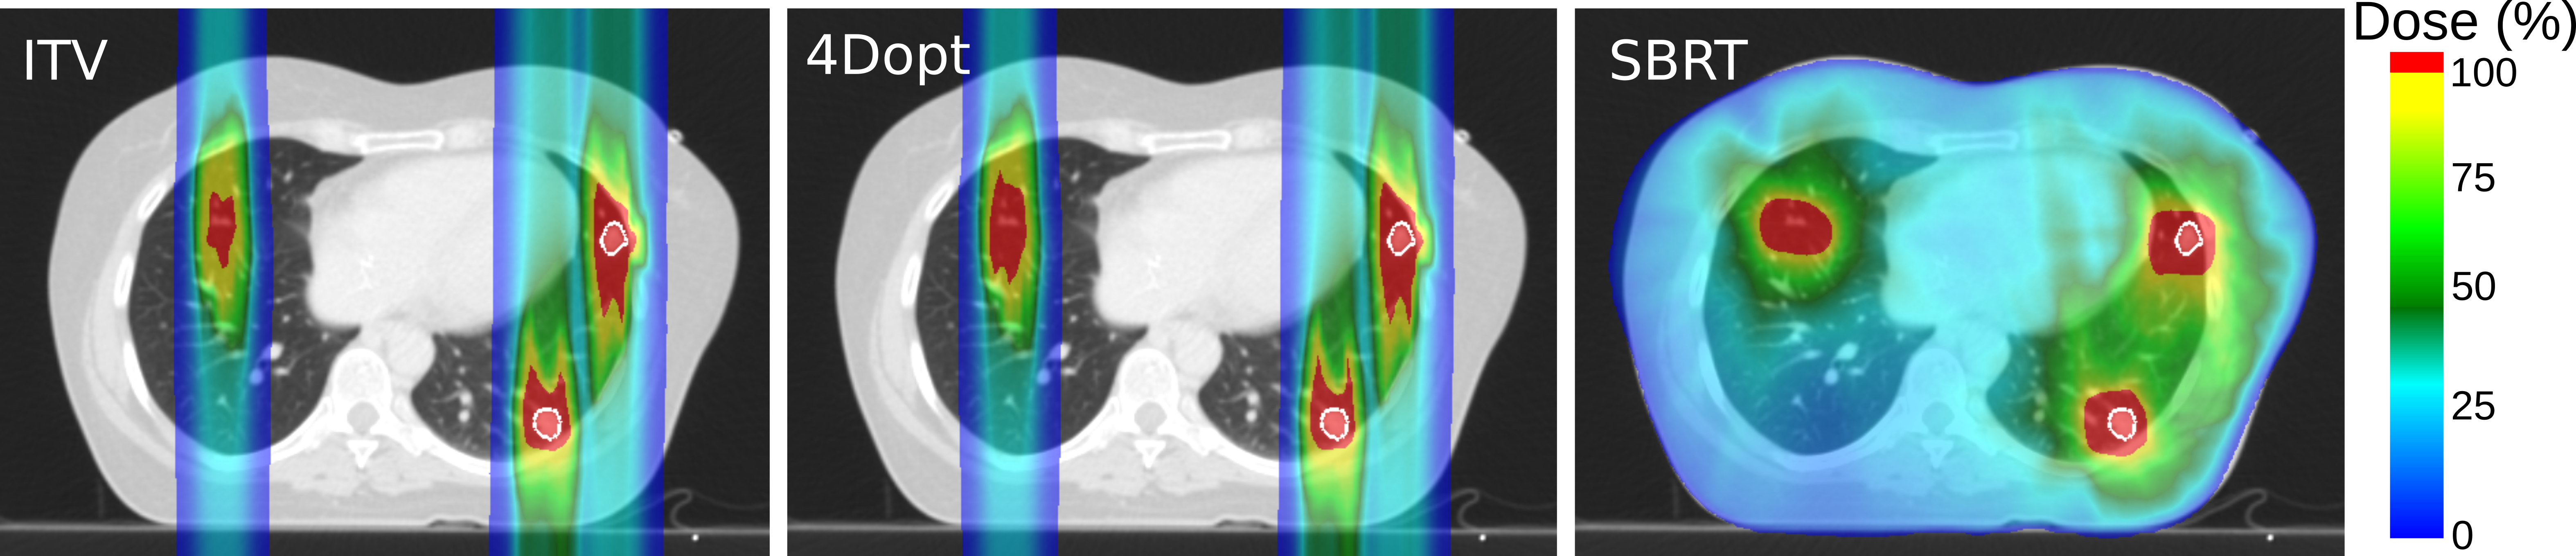
\includegraphics[width=0.9\textwidth]{./Images/multiExample.png}
		\caption{Treatment plans for indITV (left), 4Dopt (middle) and SBRT (right) for SBRT (solid lines) on a same patients. CTV contours are outlined in white.}
		\label{Fig:multiExample}
	\end{center}
\end{figure}

\subsection{Target Coverage}

Results for CTV D$_{99\%}$ for all patients are shown in Table~\ref{tab:resultsComplex}. All SBRT plans were approved by a physician, 
even though the prescription dose for patients 6 - 8 was not met, due to the OAR proximity. Excluding patients 6 - 8, there were 8  cases of too low CTV dose accross different
motion types for SFUD, indITV and 4Dopt, respectively, but not for the same targets.
For patients 6 - 8 treatment plans with SFUD were clinically unacceptable, due to violation of OAR constraints. Both indITV and 4Dopt had higher CTV D$_{99\%}$ than SBRT, while still adhearing
to OAR constraints. 

Range of CTV D$_{99\%}$ accross different motion types was 2, 1 and 2 Gy for SFUD, indITV and 4Dopt, respectively, \textbf{Statistical difference?}

\begin{table}[H]
	\centering
	%   \footnotesize
	\caption{CTV $D_{99\%}$ for indITV, 4Dopt and SBRT for 8 patients. Results for indITV and 4Dopt are shown as median (range) across different motion types.}
	\begin{tabular}{c|c|c|c|c}
		\hline\hline
		\multirow{2}{*}{Patient} & \multirow{2}{*}{Target} & \multicolumn{3}{|c}{CTV $D_{99\%}$} (\%) \\
		 &  & indITV & 4Dopt & SBRT \\
		 \hline
		 
\multirow{2}{*}{1} & a & 101.6(100.0 - 102.1) & 101.0(101.0 - 101.0) & 100.0\\ 
 & b & 101.6(101.0 - 102.1) & 102.1(101.0 - 102.1) & 100.0\\ 
\hline

\multirow{5}{*}{1} & a & 100.9(100.9 - 101.9) & 100.9(100.0 - 100.9) & 105.6\\ 
 & b & 101.3(98.8 - 102.5) & 102.5(100.0 - 102.5) & 105.0\\ 
 & c & 101.4(100.0 - 101.9) & 99.5(99.1 - 100.0) & 106.5\\ 
 & d & 100.6(100.0 - 101.3) & 98.8(98.8 - 101.3) & 112.5\\ 
 & e & 102.5(100.0 - 102.5) & 102.5(101.3 - 102.5) & 101.3\\ 
\hline

\multirow{2}{*}{1} & a & 101.0(100.0 - 101.0) & 100.5(100.0 - 101.0) & 101.0\\ 
 & b & 107.1(103.6 - 107.1) & 100.0(100.0 - 103.6) & 100.0\\ 
\hline

\multirow{5}{*}{1} & a & 101.0(99.0 - 102.1) & 99.0(99.0 - 102.1) & 106.3\\ 
 & b & 102.1(99.0 - 102.1) & 102.1(102.1 - 102.1) & 103.1\\ 
 & c & 101.0(101.0 - 102.1) & 101.6(101.0 - 102.1) & 104.2\\ 
 & d & 102.1(99.0 - 102.1) & 101.6(101.0 - 102.1) & 107.3\\ 
 & e & 102.1(102.1 - 102.1) & 102.1(101.0 - 102.1) & 108.3\\ 
\hline

\multirow{2}{*}{1} & a & 102.1(102.1 - 102.1) & 102.1(102.1 - 102.1) & 101.0\\ 
 & b & 99.0(99.0 - 99.0) & 100.0(100.0 - 101.0) & 102.1\\ 
\hline

\multirow{2}{*}{1} & a & 84.3(82.4 - 85.2) & 69.0(68.5 - 69.4) & 66.7\\ 
 & b & 100.5(99.0 - 102.1) & 100.5(99.0 - 102.1) & 103.1\\ 
\hline

\multirow{4}{*}{1} & a & 100.5(100.0 - 102.1) & 99.5(99.0 - 101.0) & 101.0\\ 
 & b & 100.5(100.0 - 101.0) & 100.0(100.0 - 100.0) & 101.0\\ 
 & c & 91.1(88.5 - 92.7) & 92.7(86.5 - 93.8) & 99.0\\ 
 & d & 97.4(93.8 - 100.0) & 100.0(99.0 - 101.0) & 94.8\\ 
\hline

\multirow{2}{*}{1} & a & 87.5(86.5 - 89.6) & 94.3(92.7 - 94.8) & 69.8\\ 
 & b & 79.7(79.2 - 81.3) & 78.6(77.1 - 79.2) & 69.8\\ 
\hline

		
		\hline




		\hline
		
% 		\hline\hline
	\end{tabular}
	\label{tab:resultsComplex}
\end{table}

% \newpage
% 
% \begin{table}[H]
% 	\centering
% 	%   \footnotesize
% 	\caption{Target characteristics, with CTV volumes, peak-to-peak motions, fractination schemes and number of fields used for treatment planning.}
% 	\begin{tabular}{c|c|c|c|c|c}
% 		\hline\hline
% 		\multirow{2}{*}{Patient} & \multirow{2}{*}{Target} & \multicolumn{4}{|c}{D$_{99\%}$} \\
% 		 & & SFUD & indITV & 4Dopt & SBRT \\
% 		\hline
% \multirow{2}{*}{1} & a & 101.0(100.0 - 101.0) & 101.0(100.0 - 102.1) & 101.0(101.0 - 101.0) & 100.0\\ 
%  & b & 102.1(102.1 - 102.1) & 101.6(101.0 - 102.1) & 101.0(101.0 - 102.1) & 100.0\\ 
% \hline
% 
% \multirow{5}{*}{1} & a & 104.2(101.9 - 105.6) & 100.9(100.0 - 101.9) & 100.0(99.1 - 100.0) & 100.9\\ 
%  & b & 101.9(101.3 - 103.8) & 100.6(98.8 - 101.3) & 101.3(100.0 - 101.3) & 92.5\\ 
%  & c & 114.4(113.9 - 114.8) & 100.9(100.0 - 101.9) & 99.1(98.1 - 100.0) & 106.5\\ 
%  & d & 98.1(97.5 - 98.8) & 100.0(98.8 - 101.3) & 98.1(97.5 - 100.0) & 112.5\\ 
%  & e & 101.3(101.3 - 101.3) & 102.5(100.0 - 102.5) & 101.3(101.3 - 102.5) & 81.3\\ 
% \hline
% 
% \multirow{2}{*}{1} & a & 99.5(95.8 - 101.0) & 100.0(99.0 - 101.0) & 100.0(100.0 - 100.0) & 101.0\\ 
%  & b & 96.4(92.9 - 103.6) & 103.6(100.0 - 103.6) & 100.0(100.0 - 103.6) & 100.0\\ 
% \hline
% 
% \multirow{5}{*}{1} & a & 99.5(97.9 - 100.0) & 100.5(99.0 - 101.0) & 97.9(97.9 - 100.0) & 106.3\\ 
%  & b & 100.0(100.0 - 100.0) & 102.1(94.8 - 102.1) & 101.0(101.0 - 101.0) & 103.1\\ 
%  & c & 100.5(100.0 - 101.0) & 100.5(99.0 - 102.1) & 101.0(100.0 - 101.0) & 104.2\\ 
%  & d & 94.3(93.8 - 94.8) & 102.1(95.8 - 102.1) & 101.0(101.0 - 101.0) & 107.3\\ 
%  & e & 94.8(94.8 - 94.8) & 100.5(100.0 - 101.0) & 100.0(99.0 - 100.0) & 108.3\\ 
% \hline
% 
% \multirow{2}{*}{1} & a & 102.1(102.1 - 102.1) & 100.0(100.0 - 100.0) & 100.0(100.0 - 100.0) & 101.0\\ 
%  & b & 97.4(96.9 - 97.9) & 96.9(96.9 - 97.9) & 94.8(94.8 - 94.8) & 102.1\\ 
% \hline
% 
% \multirow{2}{*}{1} & a & 84.3(83.3 - 85.2) & 72.7(72.2 - 73.1) & 56.0(55.6 - 56.5) & 0.0\\ 
%  & b & 82.8(80.2 - 85.4) & 100.0(96.9 - 101.0) & 99.0(99.0 - 99.0) & 101.0\\ 
% \hline
% 
% \multirow{4}{*}{1} & a & 101.0(99.0 - 102.1) & 100.0(99.0 - 101.0) & 97.4(96.9 - 97.9) & 101.0\\ 
%  & b & 106.8(105.2 - 107.3) & 97.9(96.9 - 99.0) & 96.4(95.8 - 96.9) & 101.0\\ 
%  & c & 97.9(97.9 - 99.0) & 69.3(68.8 - 70.8) & 66.7(63.5 - 68.8) & 85.4\\ 
%  & d & 100.0(99.0 - 101.0) & 71.9(70.8 - 72.9) & 72.9(70.8 - 75.0) & 83.3\\ 
% \hline
% 
% \multirow{2}{*}{1} & a & 85.9(85.4 - 86.5) & 69.3(68.8 - 70.8) & 72.9(72.9 - 74.0) & 58.3\\ 
%  & b & 68.2(66.7 - 69.8) & 62.0(60.4 - 62.5) & 57.3(57.3 - 58.3) & 53.1\\ 
% \hline
% 
% 		
% 		\hline
% 	\end{tabular}
% 	\label{tab:resultsComplex2}
% \end{table}

\subsection{Dose in OARs}

D$_{Max}$ and D$_{Mean}$ for 8 OARs are shown in Table~\ref{tab:OARComplex}. There was significant difference for \textbf{???} between PT and SBRT. No significant difference was observed for dose to OAR between different motion types.

DVHs for patients 6 - 8 are shown in Fig.~\textbf{Do it!}. SA, Es were substracted from for substracion from target were ..., compared to 2 mm in SBRT
SA D$_{Max}$ limit was exceeded for patients 6 and 8 in all cases. Heart D$_{Max}$ limit was exceeded in 1, 2 and 0 different motion cases for SFUD, indITV and 4Dopt, respectively.


\begin{table}[H]
	\centering
	%   \footnotesize
	\caption{Target characteristics, with CTV volumes, peak-to-peak motions, fractination schemes and number of fields used for treatment planning.}
	\begin{tabular}{c|c|c|c|c}
		\hline\hline
		OAR & SFUD & indITV & 4Dopt & SBRT \\
		\hline
heart & 0.4(0.0 - 1.1) & 0.3(0.0 - 0.8) & 0.4(0.0 - 1.0) & 4.4(2.5 - 10.1)  \\ 
spinalcord & 0.0(0.0 - 0.7) & 0.0(0.0 - 0.5) & 0.0(0.0 - 0.6) & 1.8(0.8 - 2.5)  \\ 
smallerairways & 0.3(0.0 - 10.4) & 1.1(0.0 - 8.2) & 1.2(0.0 - 10.3) & 3.5(0.0 - 7.5) \\ 
esophagus & 0.1(0.0 - 1.5) & 0.1(0.0 - 1.4) & 0.1(0.0 - 1.8) & 3.3(1.4 - 5.1)  \\ 
trachea & 0.0(0.0 - 0.1) & 0.0(0.0 - 0.0) & 0.0(0.0 - 0.1) & 0.1(0.0 - 3.0)  \\ 
aorta & 0.5(0.0 - 1.1) & 0.4(0.0 - 1.0) & 0.5(0.0 - 0.8) & 2.9(1.3 - 6.2)  \\ 
lungl & 3.5(0.1 - 11.0) & 3.0(0.0 - 9.1) & 3.0(0.1 - 8.6) & 5.9(0.9 - 10.5)  \\ 
lungr & 2.0(0.0 - 3.3) & 1.8(0.0 - 6.0) & 1.9(0.0 - 5.6) & 3.0(0.8 - 8.6)  \\ 

\hline\hline

heart & 14.1(0.0 - 39.3) & 13.9(0.0 - 28.5) & 14.6(0.0 - 29.3) & 18.1(7.5 - 30.5)\\ 
spinalcord & 0.4(0.0 - 8.0) & 0.4(0.0 - 8.3) & 0.3(0.0 - 8.5) & 9.0(3.0 - 12.5)\\ 
smallerairways & 14.1(0.0 - 26.0) & 13.5(0.0 - 24.0) & 13.8(0.0 - 27.5) & 15.6(0.0 - 22.8)\\ 
esophagus & 0.6(0.0 - 23.8) & 0.6(0.0 - 23.5) & 1.0(0.0 - 26.0) & 11.5(5.5 - 25.5)\\ 
trachea & 0.0(0.0 - 3.8) & 0.0(0.0 - 1.3) & 0.0(0.0 - 5.0) & 0.4(0.0 - 7.5)\\ 
aorta & 6.9(2.0 - 35.8) & 4.6(0.0 - 28.5) & 6.5(1.5 - 26.5) & 18.1(6.3 - 31.0)\\ 
lungl & 26.8(8.0 - 52.3) & 27.1(0.0 - 31.5) & 26.6(8.0 - 29.8) & 26.5(10.0 - 32.3)\\ 
lungr & 26.0(0.3 - 30.5) & 25.8(0.5 - 34.8) & 26.1(0.3 - 29.0) & 26.1(3.8 - 30.0)\\ 
\hline\hline

	\end{tabular}
	\label{tab:OARComplex}
\end{table}


\section{Summary and Discussion}

Clinically valid SBRT plans have been compared to PT treatment plans for NSCLC patients with multiple metastases. To the best of our knowledge, this is the first study of treating multiple NSCLC metastases. Novel approch was used to handle multiple targets, together
with state of the are 4D PT treatment planning. Furthermore, 4D doses were calculated for PT treatment plans. PT on average delievered less dose to OAR, while there were no
significant difference in target coverage. The most apperent difference is in lung V_${20\%}$, which was 3333\% lower in PT, due to the narrow entry channel PT use.

Patients 1 - 5 did not require OAR implementation in optimization and nevertheless no OAR constraints were violated. Even though patient 2 and 4 had 5 metastases each. For patients 1 - 5 the OARs were at least 10 mm away from the CTV, whereas for
patient 6 - 8 they were closer than 10 mm. The optimization problem was therefore more complex, especially in 4Dopt case. Patient 6 had the best target coverage with indITV, however $D_{Max}$ for smaller airways was exceeded. For patient 7 PT and SBRT target
coverage and heart $D_{Max}$ were similar, but PT delivered less dose to other OAR. Patient 8 ?


\textbf{Comparison between 4dopt and inditv}

Even though carbon-ions exhibit less dose to OAR with the same or even better target coverage, there is still room for improvement in PT treatment planning. An implementation of multi-criteria objective planning should bring
even better dose distribution and allow physician to choose between trade-offs  \cite{Breedveld2007, Chen2010}. Additionally, multiple target optimization in PT would benefit from a shell around PT where dose would be minimized. Therefore excessive dose
in healthy tissue would be further reduced. An introduction of a shell, however, would further enlarge the optimization problem, which is large already for complex geometry (patient 6 - 8). A solution for minimizing voxel number in optimization is
currently being implemented by Prall et al \textbf{Citat, mogoce mal vec napisat.} 

In Chapter~\ref{PatStudy} additional range margins could be used in treatment planning, because a single-field uniform dose (SFUD) optimization was done. Instead of defining margins in PTV, a solution was proposed to include uncertainties, such as range errors, 
in optimization process itself \cite{Pflugfelder2008, Unkelbach2009, Fredriksson2011, Chen2012}. Chen et al. have shown it is possible to implement robust optimization in multi-criteria optimization as well. 

Patient 7 $D_{Max}$ heart dose was over and under the limit across different motion types. This shows the necessity of making treatment plans robust against motion uncertainty, especially in the hypo-fractionated treatment. A recent treatment planning study by Liu et al. \cite{Liu2016}
showed a 4D robust optimization had better results than 3D robust optimization for NSCLC patients. However, only breathing starting phase was used as an uncertainty, whereas different motion types should be considered. The disadvantage of 3D and 4D robust optimization is the enlargement of 
optimization problem.

Effect of motion on treatment plan delivery could be reduced by using gating. Gating, together with rescanning, has already been successfully implemented clinically for active beam scanning \cite{Rossi2016, Mori2016} and it might be essential to use it in hypo-fractionated 
treatment of moving tumors.

A recent review showed good local control rates between 66 - 92\% for patients treated with SBRT in reoccurred tumors in previous irradiation field \cite{Amini2014}. 
However, there were grade 4 and 5 complications present, i.e. study by Trovo et al showed grade 5 pneumonia in
6\% of patient treated \cite{Trovo2014}. As shown in our study, PT delivers less dose to the OAR and could hence reduce the number of complications.

\section{Conclusions}

PT delivers less dose to OAR compared to SBRT in NSCLC patients with multiple disease sites, while maintaining the same target coverage. Caution has to be taken in patients with OAR in CTV vicinity (less than 10 mm), where doses to OAR differ across different motion types.




\bibliographystyle{apalike}
\bibliography{../ref.bib}{}
% \bibliographystyle{plain}

\end{document}